\documentclass[12pt,a4paper]{article}
\usepackage[english]{babel}
\usepackage[utf8]{inputenc}
\usepackage{fancyhdr}
\usepackage{hyperref}


% Math
\usepackage{bm}

% graphics
\usepackage{graphicx}
\graphicspath{ {images/} }
\usepackage{tikz}

% date
\usepackage{datetime}
\newdateformat{specialdate}{\THEYEAR-\twodigit{\THEMONTH}-\twodigit{\THEDAY}}
\date{\specialdate\today}
\usepackage{xcolor}

% Colors
\definecolor{command}{rgb}{0.325, 1, 1}
\definecolor{flag}{rgb}{1, 0.325, 0.325}
\definecolor{param}{rgb}{0.825, 0.825, 0.825}

%renew commands
\renewcommand{\contentsname}{Tabla de contenidos}

\begin{document}
	\begin{titlepage}
		\centering
		
\includegraphics[width=0.4\textwidth]{logo-ugr.png}\\*
		{\scshape\LARGE Universidad de Granada \par}
		{\large \date{\specialdate\today}\par}
		\vspace{1cm}
		{\LARGE\bfseries Práctica 4\par}
		\vspace{1.5cm}
		{\scshape\large Ingeniería de Servidores\par}
		\vspace{2cm}
		{\Large\itshape Lukas Häring García 3ºC\par}
	\end{titlepage}
	
	\tableofcontents
	
	\newpage
	
	
	%\begin{figure}[h]
	%	\centering
	%	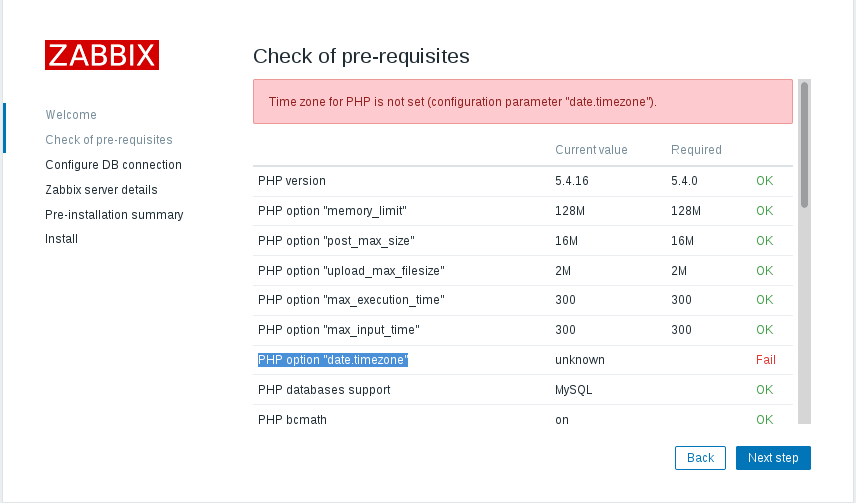
\includegraphics[width=1.0\textwidth]{images/timezone.png}
	%	\caption{Error date.timezone}
	%\end{figure}
	
	%\begin{tikzpicture}[node distance=-0.5em]
	%\node[anchor=north,draw=black,fill=black,inner xsep=0.5cm,inner ysep=0.2cm,line width=4pt,text width=\textwidth - 1cm,align=left] (box) { {\color{command}\textbf{cat}} {\color{param} /var/log/audit/audit.log} {\color{flag} $\mid$} {\color{command}\textbf{grep}} {\color{param} zabbix\_agentd} {\color{flag} $\mid$} {\color{command}\textbf{grep}} {\color{param} denied} {\color{flag} $\mid$} {\color{command}\textbf{audit2allow}} {\color{flag} -M} {\color{param} zabbix\_agent\_setrlimit}};
	%\node[fill=black,rounded corners] at (box.west) {\color{white}$\boldsymbol{>}$};
	%\end{tikzpicture}
	
	
	\section{JMeter}
	Apache JMeter es un software de código abierto, diseñada para cargar el comportamiento funcional de las pruebas y medir el rendimiento.
	
	\subsection{Instalación Ubuntu Server}
	
	Suponiendo que tenemos la \textbf{primera práctica} acabada.
	\newline
	\newline
	
\begin{tikzpicture}[node distance=-0.5em]
	\node[anchor=north,draw=black,fill=black,inner xsep=0.5cm,inner ysep=0.2cm,line width=4pt,text width=\textwidth - 1cm,align=left] (box) { {\color{command}\textbf{cat}} {\color{param} /var/log/audit/audit.log} {\color{flag} $\mid$} {\color{command}\textbf{grep}} {\color{param} zabbix\_agentd} {\color{flag} $\mid$} {\color{command}\textbf{grep}} {\color{param} denied} {\color{flag} $\mid$} {\color{command}\textbf{audit2allow}} {\color{flag} -M} {\color{param} zabbix\_agent\_setrlimit}};
	\node[fill=black,rounded corners] at (box.west) {\color{white}$\boldsymbol{>}$};
	\end{tikzpicture}
	
	\subsection{Setup en Windows}
	
	\begin{figure}[h]
		\centering
		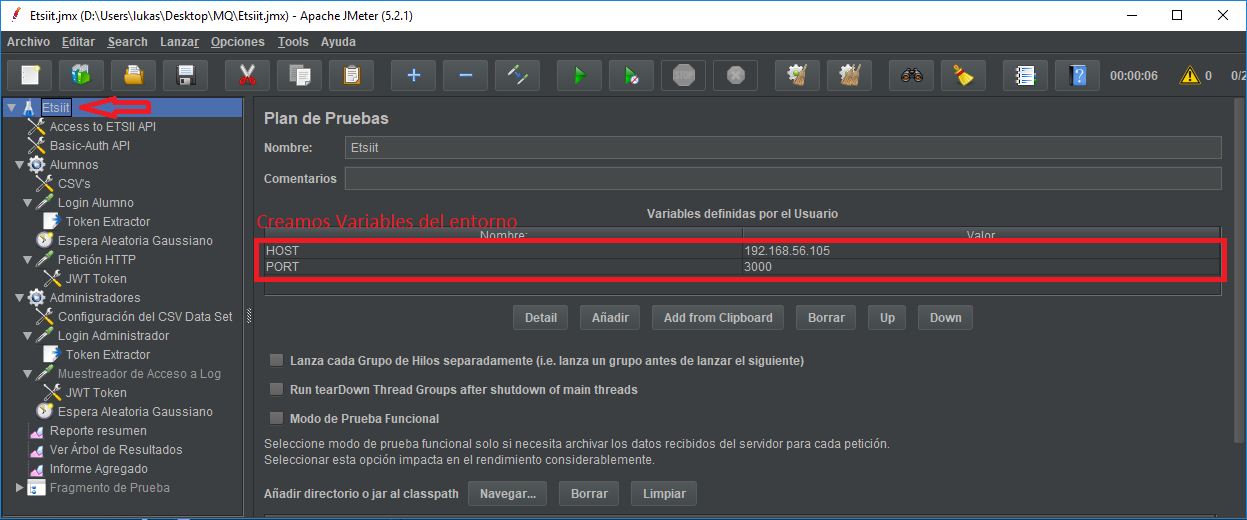
\includegraphics[width=1.0\textwidth]{images/step-1.png}
		\caption{Primer paso, creación de variables del entorno}
	\end{figure}

	\begin{figure}[h]
		\centering
		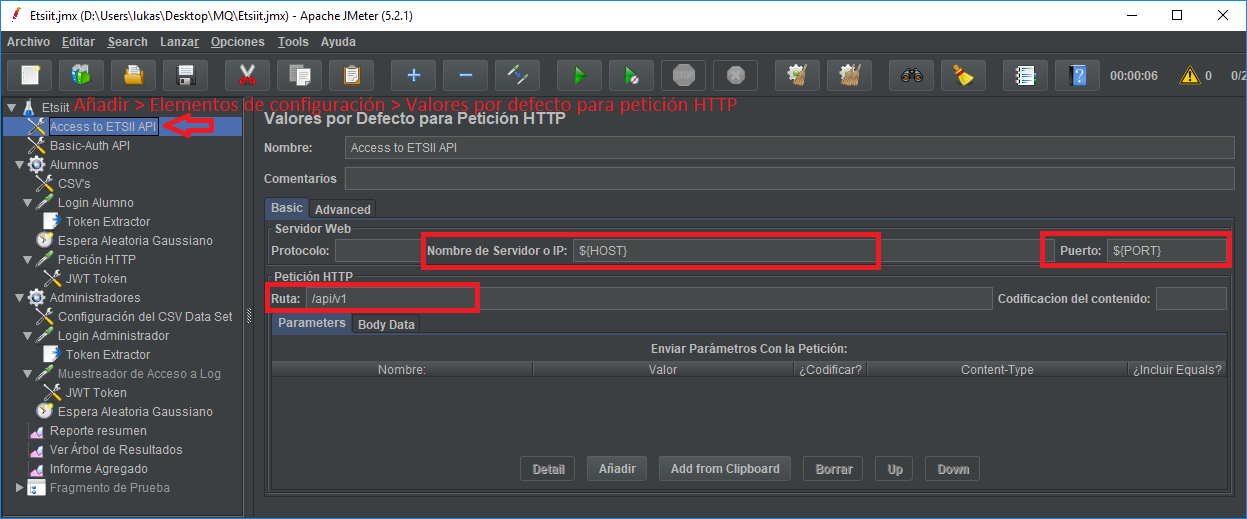
\includegraphics[width=1.0\textwidth]{images/step-2.png}
		\caption{Primer paso, creación de variables del entorno}
	\end{figure}

	\begin{figure}[h]
		\centering
		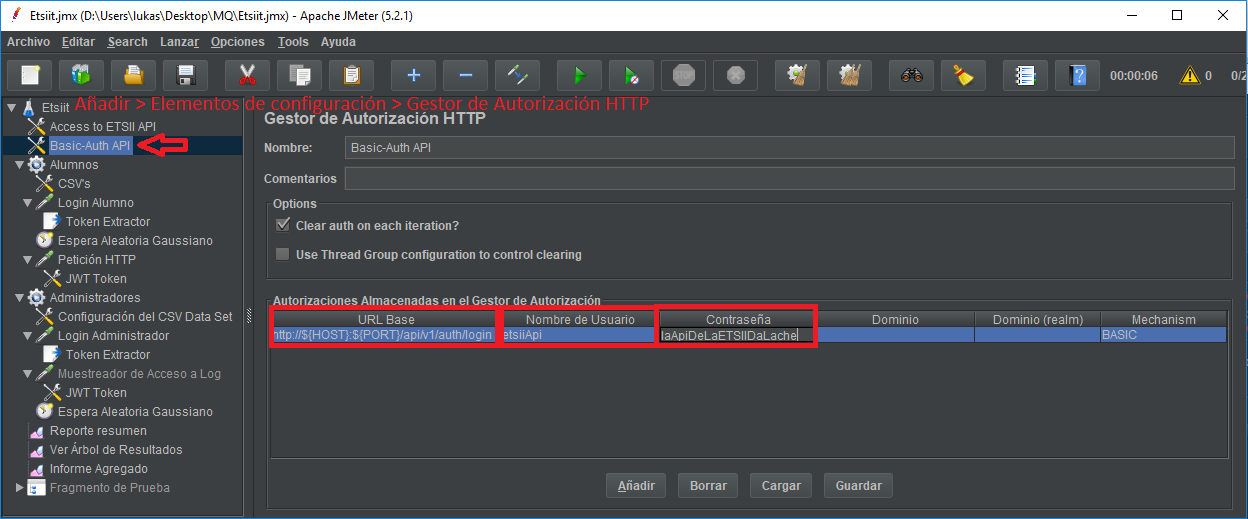
\includegraphics[width=1.0\textwidth]{images/step-3.png}
		\caption{Primer paso, creación de variables del entorno}
	\end{figure}

	\begin{figure}[h]
		\centering
		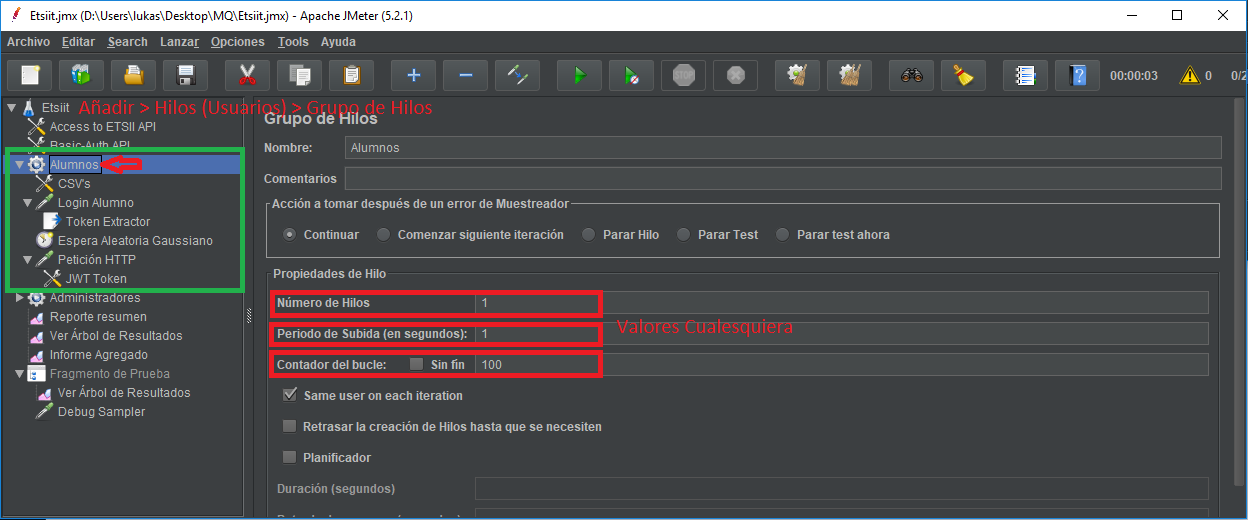
\includegraphics[width=1.0\textwidth]{images/step-4.png}
		\caption{Primer paso, creación de variables del entorno}
	\end{figure}
	
	
	\begin{figure}[h]
		\centering
		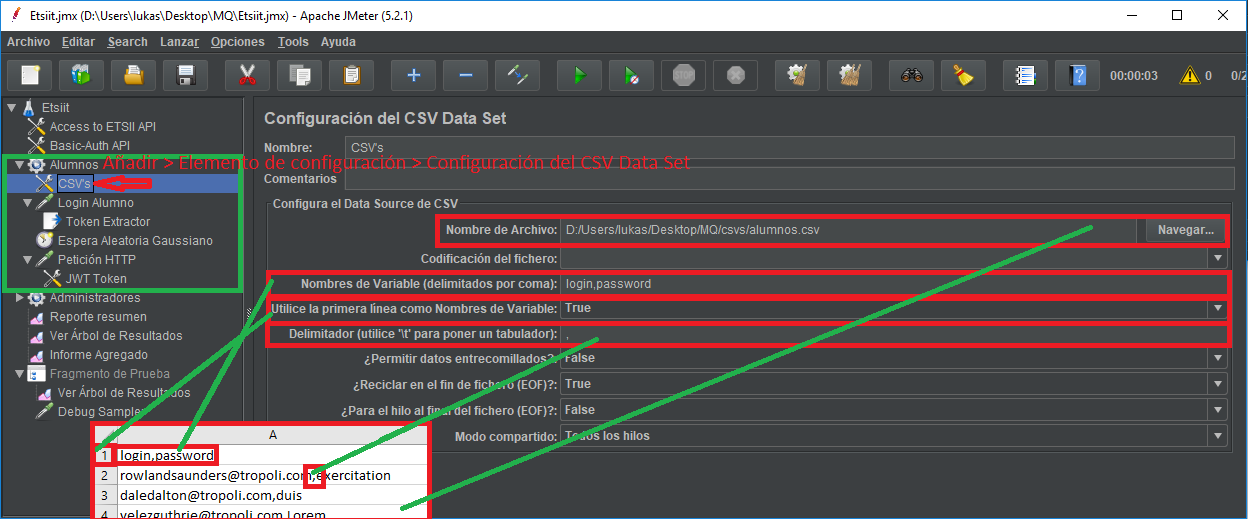
\includegraphics[width=1.0\textwidth]{images/step-5.png}
		\caption{Primer paso, creación de variables del entorno}
	\end{figure}

	\begin{figure}[h]
		\centering
		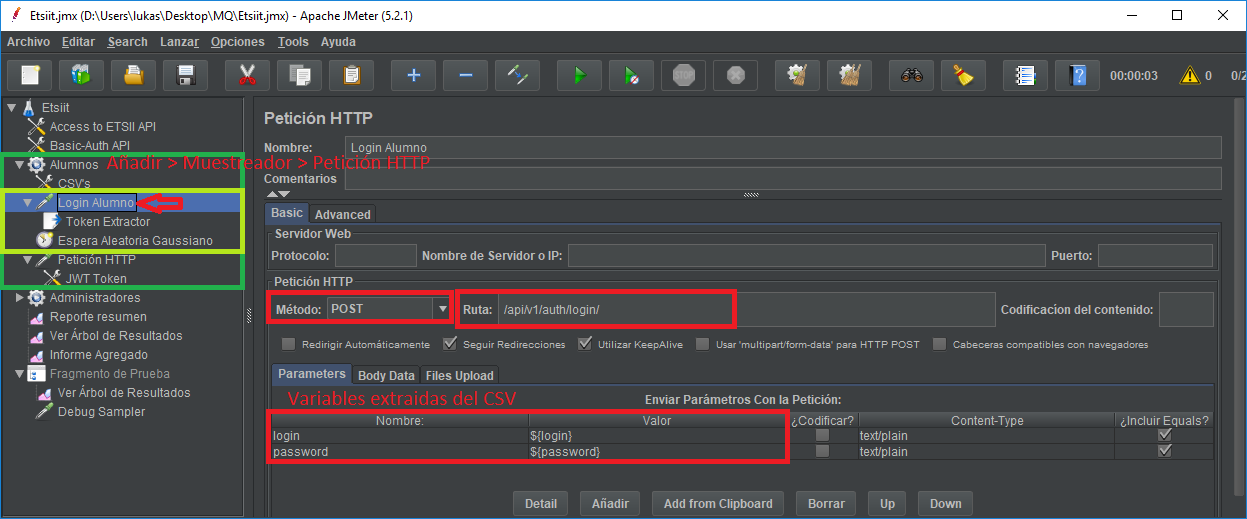
\includegraphics[width=1.0\textwidth]{images/step-6.png}
		\caption{Primer paso, creación de variables del entorno}
	\end{figure}

	\begin{figure}[h]
		\centering
		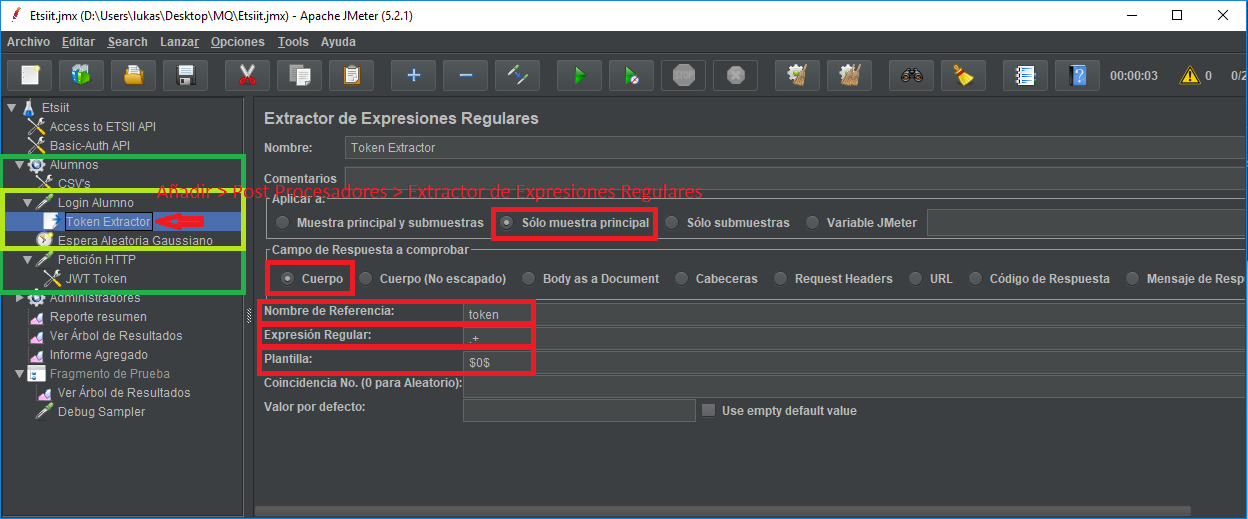
\includegraphics[width=1.0\textwidth]{images/step-7.png}
		\caption{Primer paso, creación de variables del entorno}
	\end{figure}

	\begin{figure}[h]
		\centering
		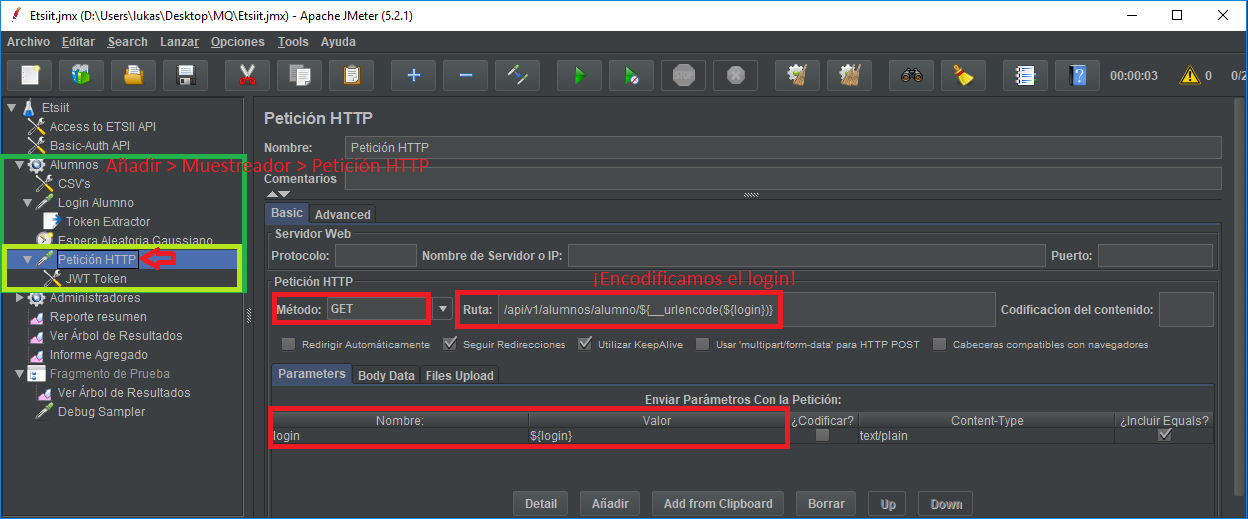
\includegraphics[width=1.0\textwidth]{images/step-8.png}
		\caption{Primer paso, creación de variables del entorno}
	\end{figure}
	\newpage
	\section{Referencias Bibliográficas}
	\begin{thebibliography}{9}
		
		%\bibitem{Zabbix}
		%¿Qué es Zabbix?
		%\url{https://es.wikipedia.org/wiki/Zabbix}
		
	\end{thebibliography}
		
\end{document}